\section{Organitzacions defensores del Programari Lliure}

Les organitzacions més influents que s'encarreguen de defensar el software lliure són:
 
 \begin{itemize}
\item \emph{Electronic Frontier Foundation}:  organitzacio sense ànim de lucre basada en part en la primera enmenda de la Constitució dels Estats Units, que defensa la llibertat d'expressió, adaptant-la als \emph{ciber-drets}, o \emph{drets virtuals}. Formada en 1990 per \textit{Mitch Kapor, John Gilmore i John Perry}, com a organització lliure vol educar a la premsa, els legisladors i el públic sobre les qüestions de llibertats civils relacionades amb les tecnologies, i actuar per a defensar-les. \cite{OrgDefEFF}
 \cite{OrgDefEFFII}
\item \emph{Free Software Foundation}: Al igual que la \emph{EFF}, és una 		organització sense ànim de lucre fundada per \emph{Richard Matthew Stallman}. És, possiblement, la organització més 		influent de programari lliure, formada alhora per una comunitat ètica en tot el món dedicada 		exclusivament al software lliure i la protecció d'aquest, dividit en diverses etapes:


	\begin{itemize}
	\item Mantenir una definició universal de programari lliure.
	\item Mantenir una educació legal sobre el FOSS, celebrant sovint seminaris sobre aspectes legals de l'ús de la 		llicència \emph{GPL} (i derivats) i oferint un servei de consulta per a advocats.
	\item Aconseguir que tothom tingui la possibilitat de \emph{tindre control sobre la tecnologia} 	quotidiana, sense restriccions de caire governamental o corporatiu. A través del desenvolupament d'un sistema operatiu completament lliure, es vol aconseguir aquest objectiu. \cite{ObjGNU} \cite{OrgDefFSF}
	\end{itemize}

\end{itemize}

\section{Casos d'èxit de Software Lliure}

\begin{itemize}

\item \emph{GNU}: va ser creat per \emph{Richard Matthew Stallman} el 1983, com a un sistema operatiu (kernel \footnote{Programa que es comunica amb els components d'un ordinador i executa i administra els recursos del mateix.} + utilitats) que es va posar en marxa per a les persones que treballaven i segueixen treballant juntes per la llibertat de tots els usuaris del programari per poder gaudir de tots els graus de llibertat d'una manera \emph{total}. Les motivacions principals que van portar a Richard a dur a terme GNU estan recollides en un document escrit per ell anomenat \emph{GNU Manifesto}. \cite{GNUExit} \cite{GNUExitII} \cite{GNUMan} \cite{GvsM}

\item \emph{Mozilla Corporation}: empresa filial propietària total de la \emph{Fundació Mozilla}, sense ànim de lucre, coordinadora i responsable de l'integració d'aplicacions informàtiques tals com el conegut navegador web \emph{Mozilla Firefox} o el client de correu electrònic \emph{Mozilla Thunderbird} en el món informàtic. Aquests programes s'actualitzen diàriament per mitja de milers de programadors voluntaris que treballen juntament amb els de la corporació que es regeixen per uns principis que l'empresa té establerts. \cite{MozExit} \cite{MozExitII} \cite{MozFesto}

\item \emph{GNU/Linux}: és un sistema operatiu lliure, format pel \emph{kernel} Linux i les utilitats del projecte GNU. Dissenyat per milers de programadors d'arreu del món, segueix en desenvolupament sota la coordinació de \emph{Linus Torvalds}. Cada dia s'actualitzen nous continguts, que milloren el funcionament del sistema operatiu. \cite{LinExit} \cite{POSIX}

\item \emph{Chromium}: és un projecte de navegador de codi obert que té com a objectiu construir una manera més segura, més ràpida i estable per a els usuaris d'experimentar amb internet. El navegador conté documents de disseny, informació de proves i altres continguts per ajudar a aprendre, construir i treballar amb el seu codi font. També es la base de \emph{Google Chrome}, la versió propietària desenvolupada per \emph{Google}. \cite{Chrom} 
\end{itemize}

\begin{figure}[ht!]
\centering
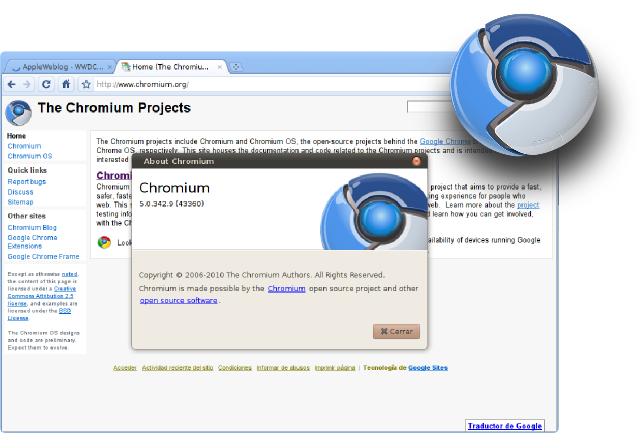
\includegraphics[width=36mm]{data/chromium.png}
\caption{Imatge del navegador lliure Chromium.}
\label{chromium}
\end{figure}